% !TeX spellcheck = ru_RU
\documentclass[a4paper,11pt, notitlepage ]{article}
\usepackage[T1]{fontenc}
\usepackage[polish]{babel}
\usepackage[utf8]{inputenc}
\usepackage{kantlipsum}
\usepackage{mwe}
\usepackage{lmodern}
\usepackage{enumitem}
\usepackage{indentfirst}
\usepackage{graphicx}
\usepackage{subcaption}
\usepackage{wrapfig}
\usepackage{fancyhdr}
\usepackage{lastpage}
\usepackage{listings}
\usepackage{spverbatim}
\usepackage{geometry}
\graphicspath{{EDSR/}{SRGAN/}}

\usepackage{listings}
\usepackage{color}

\usepackage{url}
\usepackage{hyperref}

\pagestyle{fancy}
\fancyhf{}
\rfoot{Strona \thepage  \hspace{1pt} z \pageref{LastPage}}
\lhead{Projekt dyplomowy}

\hypersetup{
	colorlinks=true,
	linkcolor=black,
	filecolor=magenta,      
	urlcolor=black,
}

\begin{document}
	
	\begin{titlepage}
		
		\newcommand{\HRule}{\rule{\linewidth}{0.5mm}} % Defines a new command for the horizontal lines, change thickness here
		
		\center % Center everything on the page
		
		%----------------------------------------------------------------------------------------
		%	HEADING SECTIONS
		%----------------------------------------------------------------------------------------
		
		\textsc{\LARGE Politechnika Warszawska}\\[1.5cm] % Name of your university/college
		\textsc{\Large Wydział Elektryczny }\\[0.5cm] % Major heading such as course name
		\textsc{\large Kierunek Informatyka }\\[0.5cm] % Minor heading such as course title
		
		%----------------------------------------------------------------------------------------
		%	TITLE SECTION
		%----------------------------------------------------------------------------------------
		
		\HRule \\[0.4cm]
		{ \huge \bfseries Wykorzystanie głębokich sieci neuronowych do poprawy rozdzielczości zdjęć twarzy. }\\[0.3cm] % Title of your document
		\HRule \\[1.5cm]
		
		%----------------------------------------------------------------------------------------
		%	AUTHOR SECTION
		%----------------------------------------------------------------------------------------
		
		\begin{minipage}{0.4\textwidth}
			\begin{flushleft} \large
				\emph{Wykonał:}\\
				Aliaksandr \textsc{Karolik} % Your name
			\end{flushleft}
		\end{minipage}
		~
		\begin{minipage}{0.4\textwidth}
			\begin{flushright} \large
				\emph{Promotor:} \\
				dr inż. Grzegorz \textsc{Sarwas} % Supervisor's Name
			\end{flushright}
		\end{minipage}\\[2cm]
		
		% If you don't want a supervisor, uncomment the two lines below and remove the section above
		%\Large \emph{Author:}\\
		%John \textsc{Smith}\\[3cm] % Your name
		
		%----------------------------------------------------------------------------------------
		%	DATE SECTION
		%----------------------------------------------------------------------------------------
		
		{\large \today}\\[2cm] % Date, change the \today to a set date if you want to be precise
		
		%----------------------------------------------------------------------------------------
		%	LOGO SECTION
		%----------------------------------------------------------------------------------------
		
		
\includegraphics[width = 28mm]{logo.jpg} % Include a department/university logo - this will require the graphicx package
		
		%----------------------------------------------------------------------------------------
		
		\vfill % Fill the rest of the page with whitespace
		
	\end{titlepage}
	\tableofcontents
	\newpage
	\section{Cel projektu}
	Praca skupiała się na badaniu najnowszych rozwiązań algorytmicznych w dziedzinie widzenia komputerowego służących do poprawy rozdzielczości, zwanych również algorytmami super-rozdzielczości (super-resolution). Wybrane metody rokujące swoją użyteczność w przypadku poprawy zdjęć twarzy zostali  zaimplementowane i przebadane.
	
	\section{Wstęp}
	Czym jest super-rozdzielczość? Super-rozdzielczość (pisana również jako super resolution, superresolution) jest określeniem zestawu metod zwiększania skali wideo lub obrazów. Terminy takie jak „skalowanie w górę”, „powiększanie”, „konwersja w górę” i „uprez” również opisują wzrost rozdzielczości w przetwarzaniu obrazu lub edycji wideo. Większość technik super-rozdzielczości opiera się na tym samym pomyśle: wykorzystanie informacji z kilku różnych obrazów do stworzenia jednego powiększonego obrazu. Algorytmy próbują wyodrębnić szczegóły z każdego obrazu w sekwencji, aby zrekonstruować inne ramki. 

	Głównym celem super-rozdzielczości jest wygenerowanie obrazu o wyższej rozdzielczości z obrazów o niższej rozdzielczości. Obraz w wysokiej rozdzielczości oferuje dużą gęstość pikseli, a tym samym więcej szczegółów na temat oryginalnej sceny. Potrzeba wysokiej rozdzielczości jest powszechna w wizji komputerowej	aplikacje dla lepszej wydajności w rozpoznawaniu wzorów i analizie obrazów. Wysoka rozdzielczość ma znaczenie w obrazowaniu medycznym dla diagnozy. Wiele aplikacji wymaga powiększenia określonego obszaru zainteresowania obrazu, w którym niezbędna jest wysoka rozdzielczość, np. aplikacje do nadzoru, kryminalistyki i obrazowania satelitarnego.
	\section{Wstęp teoretyczny}
	Super-rozdzielczość (SR) odnosi się do zadania przywracania obrazów o wysokiej rozdzielczości z jednej lub więcej obserwacji tej samej sceny w niskiej rozdzielczości (LR). Zgodnie z liczbą wejściowych obrazów LR, SR można podzielić na super-rozdzielczość pojedynczego obrazu (SISR) i super-rozdzielczość wielu obrazów (MISR). W porównaniu z MISR, SISR jest znacznie bardziej popularny ze względu na wysoką wydajność. Typowa struktura SISR, wygłąda następująco:
	\begin{figure}[h]
	\centering
	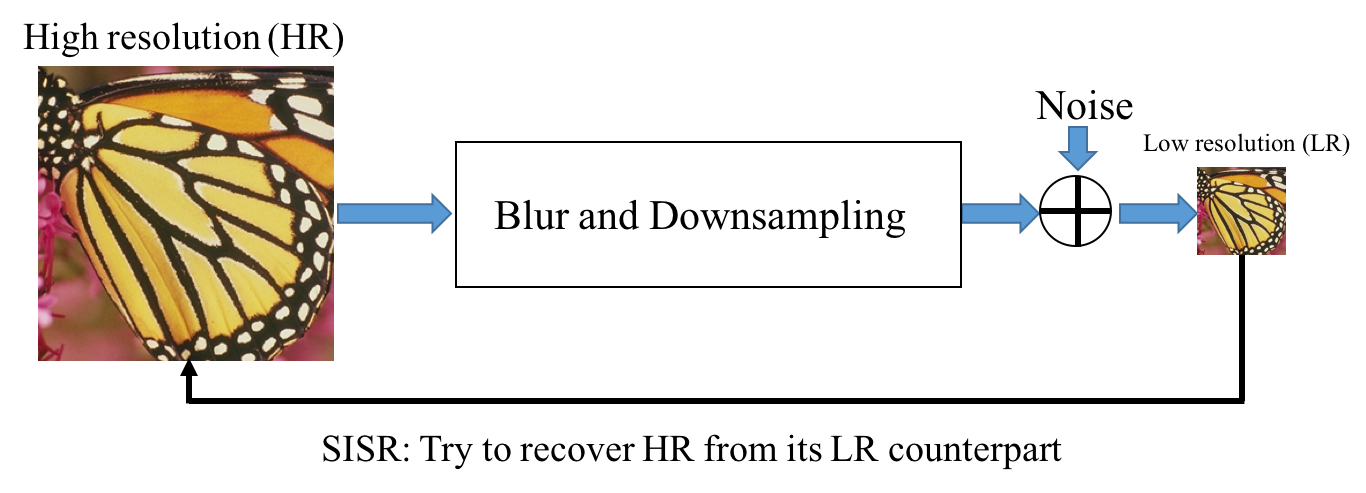
\includegraphics[width=0.7\textwidth]{sisr.png}
	\caption{Szkic SISR}
	\label{fig:mesh1}
	\end{figure}
	\newpage
	Głównie algorytmy SISR dzielą się na trzy kategorie: metody oparte na interpolacji, metody oparte na rekonstrukcji oraz metody oparte na uczeniu. Metody SISR oparte na interpolacji, takie jak interpolacja dwusześcienna (bicubic  interpolation) i próbkowanie Lanczosa (Lanczos resampling), są bardzo szybkie i proste, ale dość nie dokładne.
	  
	 Metody SR oparte na rekonstrukcji,  często przyjmują zaawansowaną wcześniejszą wiedzę w celu ograniczenia możliwej przestrzeni rozwiązań z korzyścią polegającą na generowaniu elastycznych i ostrych szczegółów. Jednak wydajność wielu metod opartych na rekonstrukcji szybko spada, gdy zwiększa się skala, oraz metody te są zwykle czasochłonne.
	 
	 Metody SISR oparte na uczeniu, znane również jako metody oparte na przykładach, najczęściej używane ze względu na ich szybkie obliczenia i wyjątkową wydajność. Metody te zwykle wykorzystują algorytmy uczenia maszynowego do analizy związków statystycznych między LR i odpowiadającym mu odpowiednikiem HR z istotnych przykładów szkoleniowych.
	 
	 Technika MISR wykorzystuję jako wejście zestaw obrazów niskiej rozdzielczości do budowy obrazu HR, ale jak już wcześniej było wspomniane, SISR jest popularniejsza ze względu na wysoką wydajność.
	 \newpage
	 \section{Metryki porównania jakości}
	 Do porównania wyników działania algorytóm zostaną wykorzystane następujące metryki:
	 \begin{itemize}
	 	\item Szczytowy stosunek sygnału do szumu (PSNR, ang. peak signal-to-noise ratio)
	 	\item Podobieństwo strukturalne (SSIM, ang. structure similarity) 
	 \end{itemize}
 	\subsection{Szczytowy stosunek sygnału do szumu}
 	Szczytowy stosunek sygnału do szumu, rzadziej stosunek sygnału szczytowego do szumu (PSNR, ang. peak signal-to-noise ratio) – stosunek maksymalnej mocy sygnału do mocy szumu zakłócającego ten sygnał. Ze względu na szeroki zakres wartości PSNR wyrażany jest w decybelach. 
 	
 	Najczęściej PSNR stosowany jest do oceny jakości kodeków wykorzystujących stratną kompresję obrazów. W takim przypadku sygnałem są nieskompresowane dane źródłowe, a szumem – artefakty (zniekształcenia) spowodowane zastosowaniem kompresji stratnej.
 	
 	W celu wyznaczenia PSNR należy wpierw obliczyć współczynnik MSE (ang. mean squared error) bazujący na obu porównywanych obrazach, korzystając z wzoru:
 	
 	$$ MSE= \frac{1}{M*N} \sum_{i=1}^{N} \sum_{j=1}^{M} ([f(i,j)-f'(i,j)]^2)$$
 	Gdzie:
 	\begin{itemize}
 		\item $N,M$ - wymiary obrazu w pikselach,
 		\item $f(i,j)$- wartość piksela o współrzędnych $(i,j)$ obrzu oryginalnego,
 		\item $f'(i,j)$- wartość piksela o wpółrzędnych $(i,j)$ obrazu skompresowanego.
 	\end{itemize}
 
 	$$PSNR= 10 log_{10}{\frac{[max(f(i,j))]^2}{MSE}}$$
 	
 	Gdzie: 
 	\begin{itemize}
 		\item $max(f(i,j))$ – wartość maksymalna danego sygnału; w przypadku obrazów zwykle jest to wartość stała, np. dla obrazów monochromatycznych o reprezentacji 8-bitowej wynosi $255$.
 	\end{itemize}
 
	\section{Podobieństwo strukturalne}
	SSIM służy do pomiaru podobieństwa pomiędzy dwoma obrazami. Indeks SSIM jest metodą pełnego porównania, innymi słowy, mierzy jakość w oparciu o oryginalny obraz (nie skompresowany lub bez zniekształceń). Wskaźnik SSIM jest rozwinięciem tradycyjnych metod, takich jak PSNR (peak signal-to-noise ratio) i standardowa metoda błędu MSE, które okazały się niezgodne z fizjologią ludzkiego postrzegania. 
	
	Indeks SSIM zawiera się w przedziale od $-1$ do $+1$. Wartość $+1$ jest osiągana tylko wtedy, gdy próbki są w pełni autentyczne. Indeks SSIM jest obliczany w różnych oknach obrazu. Miara pomiędzy dwoma oknami $x$ i $y$ o wspólnym rozmiarze $N \times N$ wynosi:
	 $$SSIM(x,y)= \frac{(2\mu_x\mu_y+c_1)(2\sigma_{xy}+c_2)}{(\mu_x^2+\mu_y^2+c_1)(\sigma_x^2+\sigma_y^2+c_2)} $$ 
 	
 	Gdzie: 
 	\begin{itemize}
 		\item $\mu_x$ wartość średnia z $x$
 		\item $\mu_y$ wartość średnia z $y$
 		\item $\sigma_x^2$ wariancja $x$
 		\item $\sigma_y^2$ wariancja $y$
 		\item $\sigma_{xy}$ kowariancja $x$ i $y$
 		\item $c_1=(k_1L)^2, c_2=(k_2L)^2$ dwie zmienne stabilizujące podział ze słabym mianownikiem
 		\item $L$ zakres dynamiki wartości pikseli 
 		\item $k_1=0.01$ i $k_2=0.03$
 	\end{itemize}
 \newpage
	 \section{Architektury dla SISR}
	 \subsection{SRCNN}
	 SRCNN(Image Super-Resolution Using Deep Convolutional Networks
	 ). Architekturę SRCNN pokazana jest na rysunku 2. Jak ustalono w wielu tradycyjnych metodach, dla uproszczenia SRCNN używa tylko komponenty luminancji do treningu. SRCNN jest trójwarstwowym CNN (Konwolucyjne sieci neuronowe), w którym znajdują się rozmiary filtrów każdej warstwy $64 \times 1 \times 9 \times 9$, $1 \times 32 \times 5 \times 5$ i $1 \times 32 \times 5 \times 5$. Dalej w omówieniu działania algorytmu będę stosować następującą notację:
	 \begin{itemize}
	 	\item $Y$ obraz o niskej rozdzielczości
	 	\item $X$ prawdiwy obraz o wysokiej rozdzielczości  
	 \end{itemize}
	 Każda warstwa odpowiada za następujące czynności:
	 \begin{enumerate}
	 	\item Wyodrębnienie i reprezentacja. Popularną strategią w rekonstrukcji obrazu  jest wyodrębnienie plastrów, a następnie reprezentowanie ich przez zestaw wstępnie przeszkolonych baz, takich jak PCA. Jest to równoważne z zawijaniem obrazu przez zestaw filtrów, z których każdy jest podstawą. W naszym sformułowaniu, włączamy optymalizację tych baz do optymalizacji sieci. Formalnie, nasza pierwsza warstwa wyrażona jest jako operacja:
	 	$$ F_1(Y)=max(0,W_1 * Y+ B_1)$$
	 	Gdize: 
	 	\begin{itemize}
	 		\item$W_1$ - odpowiedni filter
	 		\item $B_1$ - szum
	 		\item $*$ - oznacza operację zwijania (convolution operation) 
	 	\end{itemize}
	 	\item Mapowanie nieliniowe. Pierwsza warstwa wyodrębnia $n1$-wymiarową cechę dla każdego plastra. W drugiej operacji mapujemy każdy z tych $n1$-wymiarowych wektorów na $n2$-wymiarowy. Jest to równoznaczne z zastosowaniem $n2$ filtrów. Działanie drugiej warstwy jest następujące:
	 	$$F_2(Y)= max(0,W_2*F_1(Y)+B_2)$$
	 	\begin{itemize}
	 		\item$W_2$ - odpowiedni filter
	 		\item $B_2$ - szum
	 		\item $*$ - oznacza operację zwijania (convolution operation) 
	 	\end{itemize}
 		Każdy z wyjściowych $n2$-wymiarowych vektorów jest koncepcyjnie odwzorowaniem plastra o wysokiej rozdzielczości, który zostanie użyty do rekonstrukcji.
	 	\item Rekonstrukcja. Ostatecznie  plastry o wysokiej rozdzielczości są  uśredniane w celu uzyskania ostatecznego pełnego obrazu.  Uśrednianie może być traktowane jako predefiniowany filtr na zestawie map cech (gdzie każda pozycja jest "spłaszczoną" formą wektorową plastry o wysokiej rozdzielczości). Ostatnia warstwa konwolucyjną jest definiowana następująco:
	 	$$F_3(Y)=W_3*F_2(Y)+B_3$$
	 \end{enumerate}
 	\begin{figure}[h!]
 	\centering
 	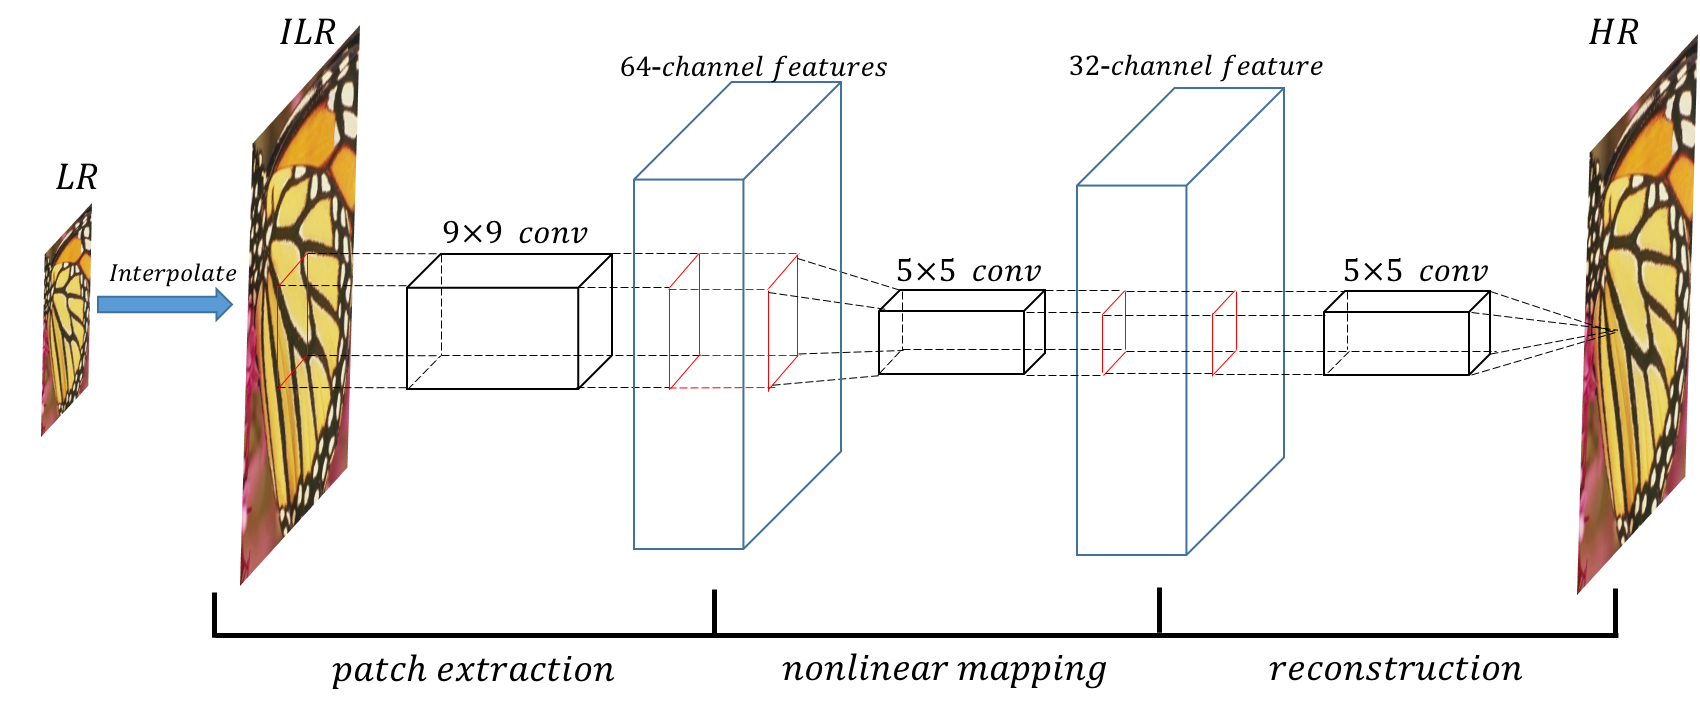
\includegraphics[width=0.8\textwidth]{SRCNN.png}
 	\caption{Architektura SRCNN.}
 	\end{figure}
 
 \newpage
	 \subsubsection{Wyniki działania algorytmu} 
	 \begin{figure}[h!]
	 	\centering
	 	\begin{subfigure}[b]{0.4\linewidth}
	 		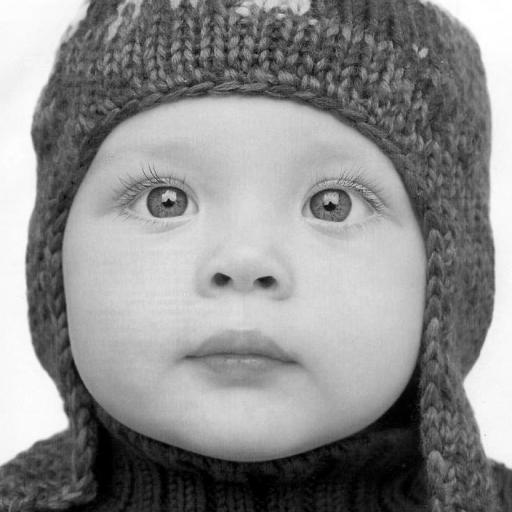
\includegraphics[width=\linewidth]{SRCNN/Input.jpg}
	 		\caption{Oryginalny obraz.}
	 	\end{subfigure}
	 	\begin{subfigure}[b]{0.4\linewidth}
	 		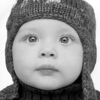
\includegraphics[width=\linewidth]{SRCNN/test_srcnn.png}
	 		\caption{Obraz  niskiej rozdzielczości.}
	 	\end{subfigure}
	 	\begin{subfigure}[b]{0.4\linewidth}
	 		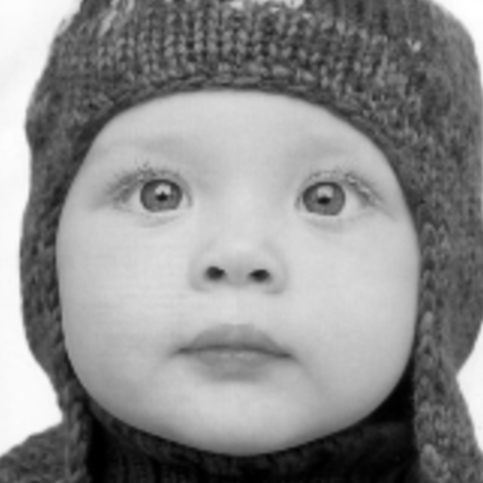
\includegraphics[width=\linewidth]{SRCNN_15000.png}
	 		\caption{Obraz wysokiej rozdzielczości.}
	 	\end{subfigure}
	 	\caption{Wyniki działania algorytmu SRCNN.}
	 	\label{fig:coffee3}
	 \end{figure}
 \newpage
 \subsection{EDSR}
 Najprostszym sposobem na zwiększenie wydajności modelu jest zwiększenie liczby parametrów. W sieci konwolucyjnej wydajność modelu może być zwiększona poprzez układanie wielu warstw lub zwiększenie liczby filtrów.

 Na Rysunku  4 (a) jest zaprezentowana użyta architektóra sieci w  EDSR (Enhanced Deep Residual Networks for Single Image Super-Resolution). Niebieskie bloki na obrazie reprezentują bloki w stylu  ResNet (ang. Residual Neural Network). Zostali one użyte ze wzgłędu na to że  super-rozdzielczość wymaga, aby większość informacji zawartych w obrazie LR została zachowana w obrazie HR. W związku z tym modele używające takie bloki uczą się głównie pozostałości między obrazami LR i HR.
 
  Autorzy stwierdzili, że zwiększenie liczby map cech powyżej pewnego poziomu spowodowałoby, że procedura szkoleniowa byłaby niestabilna pod względem obliczeniowym. Problem został rozwiązany w następujący sposób w każdym resztkowym bloku po ostatniej warstwie konwolucyjnej umieszczane są stałe warstwy skalowania. Moduły te znacznie stabilizują procedurę treningową przy użyciu dużej liczby filtrów.
 

\begin{figure}[h!]
	\centering
	\begin{subfigure}[b]{0.4\linewidth}
	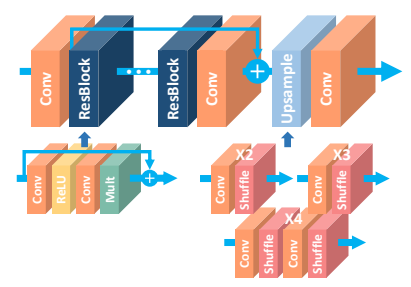
\includegraphics[width=\textwidth]{EDSR/EDSR_2.png}
	\caption{Architektura EDSR.}
	\end{subfigure}
	\begin{subfigure}[b]{0.4\linewidth}
		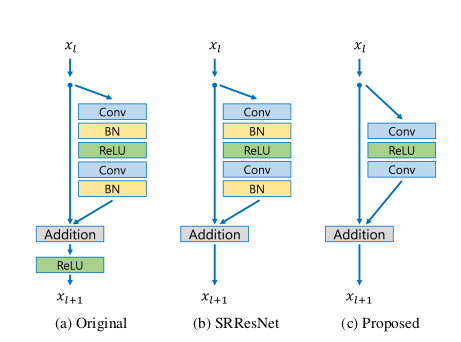
\includegraphics[width=\linewidth]{resudualbloc.png}
		\caption{Architektura ResNet oraz proponowany wariant.}
	\end{subfigure}
	\caption{Architektura EDSR.}
	\label{fig:coffee3}
\end{figure}


\newpage
 \subsubsection{Wyniki działania algorytmu}
 Poniższe wyniki powstali z wytrenowanej sieci w architektórze 16 bloków resztkowych i 64 filtrami w warstwie konwolucyjnej  filtry miały wymiar $3 \times 3$ jak jest omówione w artykule związanym z tą architektórą.
 	 \begin{figure}[h!]
 	\centering
 	\begin{subfigure}[b]{0.4\linewidth}
 		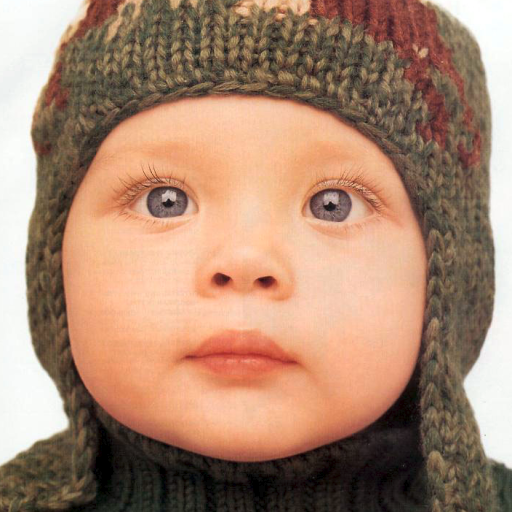
\includegraphics[width=\linewidth]{baby_GT.png}
 		\caption{Oryginalny obraz.}
 	\end{subfigure}
 	\begin{subfigure}[b]{0.4\linewidth}
 		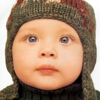
\includegraphics[width=\linewidth]{EDSR/EDSR_INPUT.png}
 		\caption{Obraz  niskiej rozdzielczości.}
 	\end{subfigure}
 	\begin{subfigure}[b]{0.4\linewidth}
 		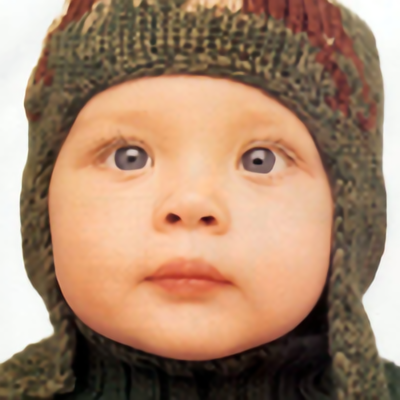
\includegraphics[width=\linewidth]{EDSR/EDSR_OUTPUT.png}
 		\caption{Obraz wysokiej rozdzielczości.}
 	\end{subfigure}
 	\caption{Wyniki działania algorytmu EDSR.}
 	\label{fig:coffee3}
 \end{figure}
\newpage
\subsection{SRGAN}
SRGAN - Photo-Realistic Single Image Super-Resolution Using a Generative AdversarialNetwork. Wybrana architektura wykorzustuje wewnątrz generatywną sieć przeciwstawną. To tak naprawdę dwie sieci neuronowe: pierwsza (generator) próbuje stworzyć obraz nieodróżnialny od prawdziwego z bazy wzorcowych danych, podczas gdy druga (dyskryminator) stara się znaleźć różnice. Ogólna idea takej architektury jest taka, że pozwala ona na szkolenie generatora w celu oszukiwania różnicującego dyskryminatora, który jest szkolony do odróżniania superrozdzielczych obrazów od rzeczywistych. Dzięki takiemu podejściu generator może nauczyć się tworzyć rozwiązania, które są bardzo podobne do prawdziwych obrazów, a przez to trudne do sklasyfikowania przez dyskryminatora. Uczenie takiego rodzaju zachęca do poszukiwania  lepszych rozwiązań  w podprzestrzeni które istneją w przestrzeni naturalnych obrazów. SRGAN jest bardziej atrakcyjny dla człowieka bo może wykreować obraz z większą ilością szczegółów. 

 Struktura sieci jest zaprezentowana na Rysunku 6.
\begin{figure}[h!]
	\centering
	\begin{subfigure}[b]{0.9\linewidth}
		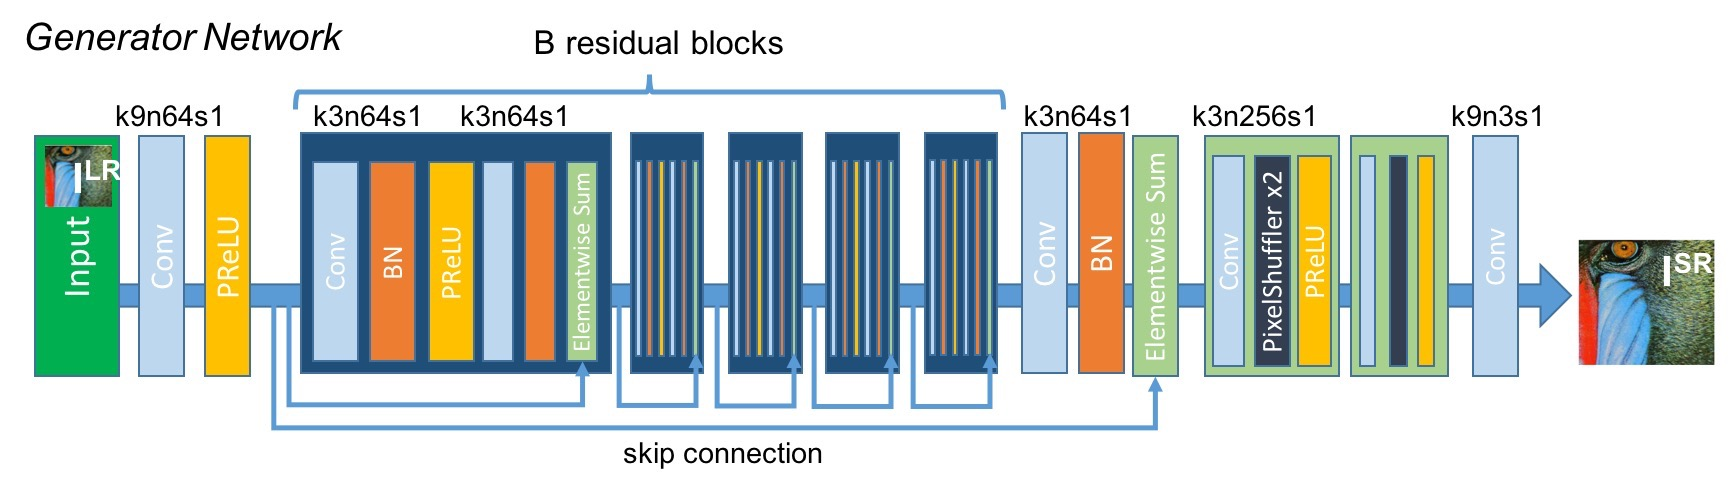
\includegraphics[width=\linewidth]{SRGAN_Generator.png}
		\caption{Architektura generatora.}
	\end{subfigure}
	\begin{subfigure}[b]{0.9\linewidth}
		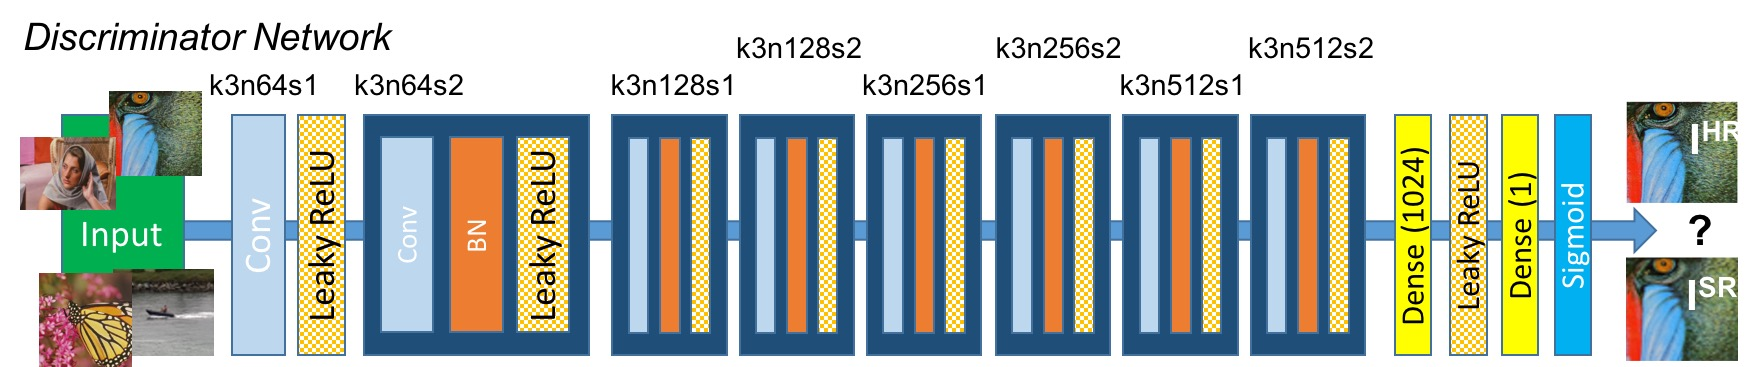
\includegraphics[width=\linewidth]{SRGAN_dyskryminator.png}
		\caption{Architektura dyskryminatora.}
	\end{subfigure}
	\caption{Architektura  SRGAN.}
	\label{fig:coffee3}
\end{figure}
\newpage
\subsubsection{Wyniki działania algorytmu}
Poniższe wyniki powstały z wytrenowanego generatora mającego 16 bloków resztkowych z 64 filtrami w warstwie konwolucyjnej  filtry miały wymiar $3 \times 3$ oraz deskryminatora który miał 8 bloków zawierających warsty konwolucyjnej każdy następny blok miał w dwa razy więcej filtrów czyli z 64 do 512.
\begin{figure}[h!]
	\centering
	\begin{subfigure}[b]{0.4\linewidth}
		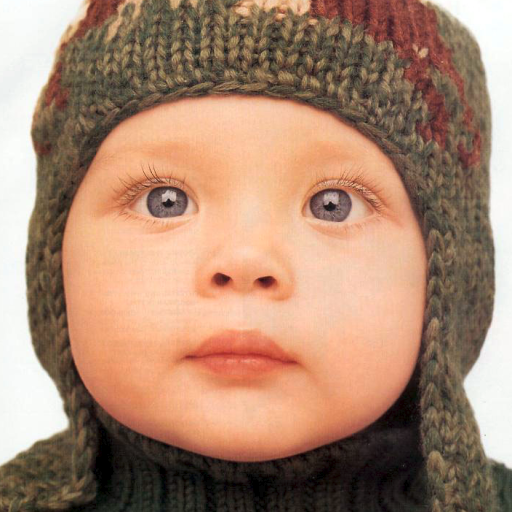
\includegraphics[width=\linewidth]{baby_GT.png}
		\caption{Oryginalny obraz.}
	\end{subfigure}
	\begin{subfigure}[b]{0.4\linewidth}
		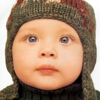
\includegraphics[width=\linewidth]{SRGAN/test.png}
		\caption{Obraz  niskiej rozdzielczości.}
	\end{subfigure}
	\begin{subfigure}[b]{0.4\linewidth}
		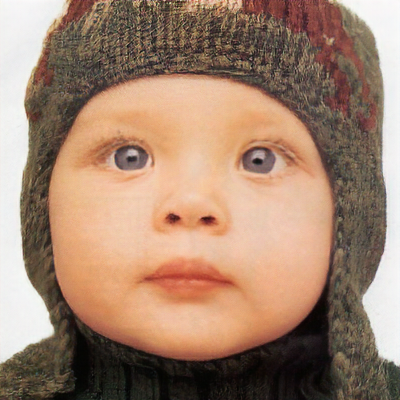
\includegraphics[width=\linewidth]{SRGAN/output_SRGAN.png}
		\caption{Obraz wysokiej rozdzielczości.}
	\end{subfigure}
	\caption{Wyniki działania algorytmu SRGAN.}
	\label{fig:coffee3}
\end{figure}
\newpage
\section{Wnisoki}

\begin{figure}[h!]
	\centering
	\begin{subfigure}[b]{0.4\linewidth}
		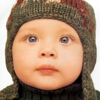
\includegraphics[width=\linewidth]{SRGAN/test.png}
		\caption{Obraz testowy.}
	\end{subfigure}
	\begin{subfigure}[b]{0.4\linewidth}
		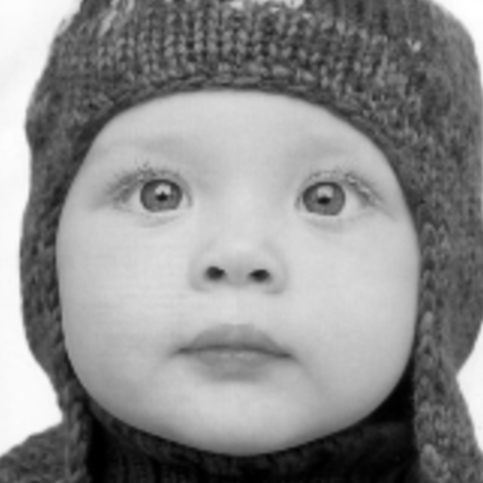
\includegraphics[width=\linewidth]{SRCNN_15000.png}
		\caption{SRCNN.}
	\end{subfigure}
	\begin{subfigure}[b]{0.4\linewidth}
		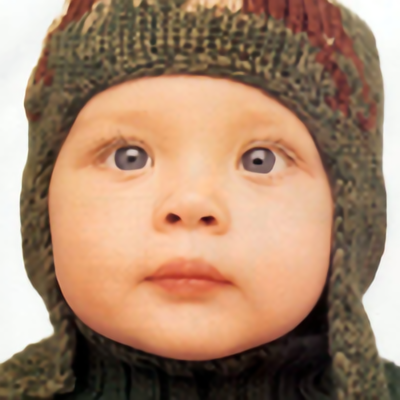
\includegraphics[width=\linewidth]{EDSR/EDSR_OUTPUT.png}
		\caption{EDSR.}
	\end{subfigure}
	\begin{subfigure}[b]{0.4\linewidth}
		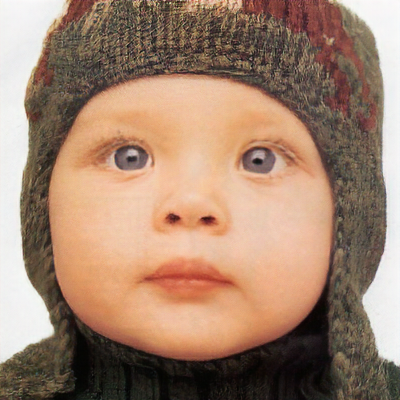
\includegraphics[width=\linewidth]{SRGAN/output_SRGAN.png}
		\caption{SRGAN.}
	\end{subfigure}
	\caption{Wyniki działania algorytmu SRGAN.}
	\label{fig:coffee3}
\end{figure}

Najlepsze wyniki osiągnął algorytm SRGAN w porównaniu z wybranymi algorytmami. Jak już było pisane wcześniej SRGAN jest bardziej atrakcyjny dla człowieka z większą ilością szczegółów wyniki eksperymentów to potwierdziły.
\newpage
\begin{thebibliography}{}
	\bibitem{litlink1}  SRCNN Image Super-Resolution Using Deep Convolutional Networks
	\url{https://arxiv.org/abs/1501.00092}
	
	\bibitem{litlink1} EDSR Enhanced Deep Residual Networks for Single Image Super-Resolution \url{https://arxiv.org/abs/1707.02921}
	
	\bibitem{litlink1} SRGAN Photo-Realistic Single Image Super-Resolution Using a Generative Adversarial Network \url{https://arxiv.org/abs/1609.04802}
	
\end{thebibliography}
\end{document}